\chapter{Ciclo de Vida}
\par O kit de automação desenvolvido pelo grupo apresenta um ciclo de vida que possui sua fase inicial de lançamento no mercado, crescimento, maturidade e declínio.

\begin{figure}[!h]
\caption{Ciclo de Vida do Projeto}
\centering
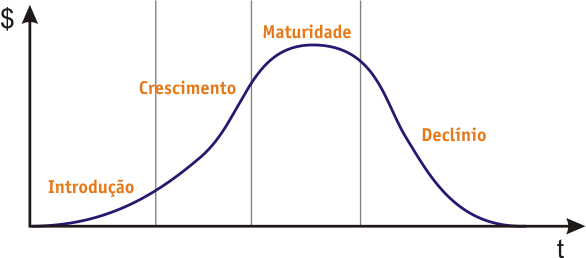
\includegraphics[width=10cm]{figuras/ciclodevida}
\end{figure}

\par O público alvo do nosso kit são consumidores de classe média e de boa estabilidade financeira, como já foi citado. A ideia dele ser introduzido no mercado é por meio de prospecção passiva que é, basicamente, o cliente procurar nosso tipo de serviço e damos a ele as opções de pacote e fechamos com ele, ou seja, a interação cliente-produto vem de iniciativa do cliente.
\par Para atingir este público serão feitas divulgações em redes sociais e possíveis parcerias com comerciantes locais de imobiliárias e lojas de elétricas e eletrônicos para disponibilização dos equipamentos, além de um site da marca para divulgação.
\par Depois do produto instalado em algumas casas, toda a sua aceitação pelo mercado a partir daí será a base de como os clientes se adaptaram ao novo estilo de vida e qualidade do serviço oferecido pelo kit.
\par Como é algo inovador o serviço deve ser apresentado de forma singela e com uma qualidade que não deixe a desejar para que o produto final perpetue no mercado.
\par Com a adesão pelos consumidores, o kit deve ganhar maior divulgação e ampliação das vendas em possíveis lojas virtuais, em nosso próprio site e sites de vendas coletivas, para garantir clientes de diferentes localidades. Também deve ser montado uma equipe de suporte para analisar possíveis erros, falhas e melhorias que podem ser feitas para melhor eficiência e conforto para o usuário.
\par Ao garantirmos uma boa aceitação no mercado e grande número de vendas, deve-se trabalhar para manter a venda e os lucros altos, pois o preço de manutenção e resolução de problemas técnicos podem fazer o lucro total diminuir.
\par Um ponto importante a se perceber é quando o kit se torna obsoleto em relação aos concorrentes ou quando a tecnologia já está ultrapassada e, assim, é necessário criar atualizar o produto e manter a assistência técnica.

\section{Recursos e Projeções Financeiras}

\par Para a realização e início do projeto seria necessário um financiamento público ou privado que permitissem seguir com o mínimo do projeto, esse financiamento seria de aproximadamente 6 vezes o valor de um projeto, para segurar a empresa nas contas e garantir um retorno econômico para os próximos. O financiamento pedido seria de R\$ 300.000,00 podendo variar até R\$ 200.000,00.
\par Após isso , se obtiver boa resposta do mercado , projetando pelo menos um lucro de 15\% no mínimo, que de acordo com Warren Buffett é um bom rendimento, por cada casa automatizada é bastante possível manter uma empresa firme e estruturada.
\par O lucro estimado com os 15\% gira em torno de R\$ 17000,00 por projeto, podendo aumentar de acordo com a taxa de lucro vista em reação ao mercado. Essa reação ascendente pode vir pela pouca concorrência e por ser um projeto pioneiro que junta duas grandes idéias.

\section{Custos}

\begin{figure}[!h]
\caption{Tabela de Custos do Projeto}
\centering
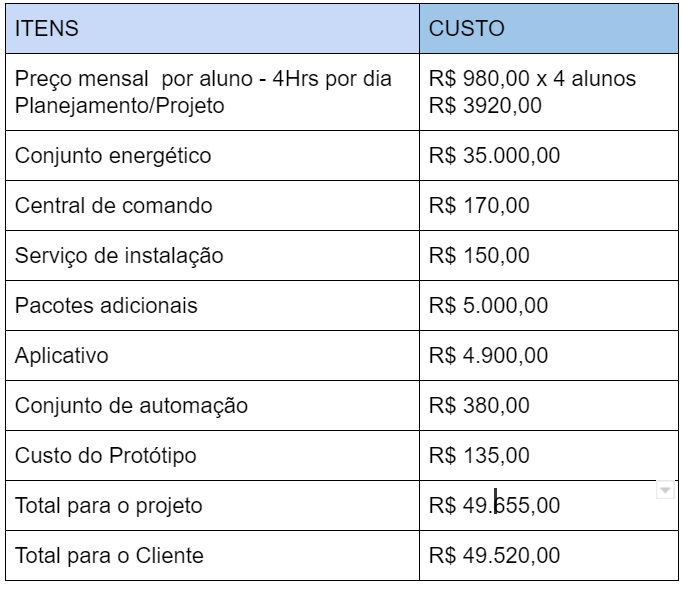
\includegraphics[width=10cm]{figuras/tabela_custos}
\end{figure}

\section{Descrição dos custos}

\par Os serviços são cobrados a partir da diária de um estudante de engenharia, que gira em torno de R\$50,00 de acordo com nossas pesquisas.
\par O preço do aplicativo é o resultado de um mês de trabalho para 5 estudantes trabalhando e testando no período de um mês.
\par O protótipo contém:
\begin{itemize}
    \item Sensor de presença (ECP  LS120E: R\$ 35,00, Loja: Leroy Merlin \-– Brasilia, DF);
    \item Câmera de segurança (Jortan Pantilt  IP: R\$ 160,00, Loja: Tudoseg \-- São José do Rio Preto, SP);
    \item Sensor de gás (HANWEI SENSORS MQ-2: R\$15,00, Loja: Curto Circuito \-- Guarulhos, SP);
    \item Central de comando (Raspberry R\$ 170,00, preço comum e fácil de achar em Brasília).
\end{itemize}

\par Os fornecedores foram escolhidos por serem um empresas renomadas no mercado, ou de confiança e um fácil acesso na região.
\par Apesar dos componentes e fornecedores já listados temos a necessidade de nos programar para imprevistos. Caso ocorram, temos outros sensores na lista que exercem a mesma função dos já escolhidos para um caso de troca, os fornecedores escolhidos também oferecem a venda dos componentes secundários escolhidos caso necessário.
\par O conjunto energético contém:

\begin{itemize}
    \item Placas solares;
    \item Medidor inteligente;
    \item Controlador de energia;
    \item Bateria;
    \item Inversores;
    \item Controlador de tensão.
\end{itemize}
